\section{Checksum Calculation}

In order to uniquely identify the files analyzed, and detect changes across runs, the Data Discovery Library must
perform some calculations on each file to generate a unique ID that is dependent on the content of the file.
Ideally these calculations are efficient and the generated IDs will have a low collision rate.

\subsection{Hashing, CRC and Checksum Algorithms}
Before deciding on the algorithm that will be used to generate the IDs, it's important to clear up the differences
between hashing, checksum and CRC algorithms.
These terms are often used interchangeably (e.g.\ the metadata generated by the library also uses the term \("\)hash\("\)
as a place-holder for the ID field)

Arguably, these operations achieve similar results, i.e.\ taking an unknown sized chunk of data, and reducing it into
a constant n-sized output value.
However, they are intended for different use cases.
The goal of a hashing algorithm is to create values that have low
collision rates, they are also often used for cryptographic applications (which is irrelevant for this project).
The low collision rates however comes at the cost of slower computation rates, compared to checksum algorithms.
The values generated by hashing algorithms are referred to as digests.

\newline

Checksum and Cyclic Redundancy Check Algorithms both aim to detect errors in the files.
Of course, by extension this
also means that files with minor changes are guaranteed to have different checksum values.
They usually have
faster computation rates compared to hashing algorithms due to their smaller sizes and lack of cryptographic concerns.
Naturally, the smaller checksum sizes do increase the chances of collisions.

The difference between CRC and checksum algorithms is the method of calculation.
CRCs are slower, but able to generate larger error runs.

\subsection{Collisions and the Birthday Problem}

Since the generated values, are meant to be used as unique identifier for files and to track changes of the files, it's important
to discuss collision rates. Figure ~\ref{fig:checksum_fig_1} shows the birthday problem in action.
Essentially, if there are 77163 files, by using a 32-bit checksum, the odds of a collision is 50%.

Therefore, there must be a careful balance between performance and coliision rates.

\begin{figure}[h]
    \centering
    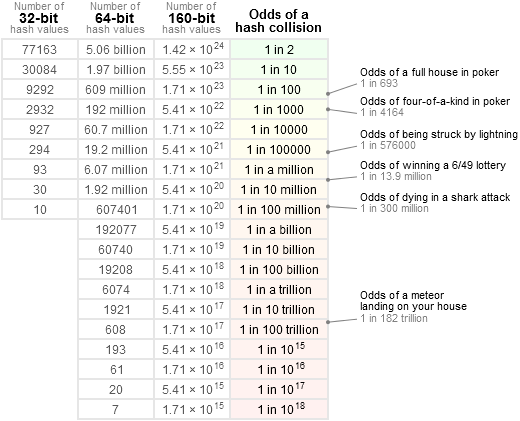
\includegraphics[width=12cm]{figures/checksum/collisions}
    \caption{Chances of collision for various bit sizes, source: ~\cite{PreshingCollisions}}
    \label{fig:checksum_fig_1}
\end{figure}



\subsection{Offloading the Hash Calculations into Compiled Modules}
Before investigating the various CRC and checksum algorithms.
It is beneficial to consider offloading the checksum calculations into a separate, compiled module.
It is easy to do so, since:

\begin{itemize}
    \item There isn't much interdependency between the checksum calculation and the rest of the library.
    \item The generated values are numeric, which are unlikely to cause conversion issues across the modules.
    \item Python has a well established culture, of offloading calculation heavy processes into compiled modules.
\end{itemize}

To test this idea, Rust was chosen as it enables its users to write low level code, while still being memory safe.
Its performance is also comparable to C. That being said, the results here are reproducible on any compiled, low level
language, assuming it can interface with Python.

The modules were always compiled with the release flag on.
The python wheels were generated using Maturin ~\cite{Maturin}.

\begin{table}[]
\begin{tabular}{ll}
Operating System  & Ubuntu 22.04.1 LTS x86\_64                                     \\
Kernel Version    & 5.15.0-56                                                      \\
Processor         & Intel i7-4700MQ @ 3.400GHz                                     \\
Memory            & 16Gb DDR3 @ 1867MHz                                             \\
Hard drive        & SATA SSD @ 452.62 MB/s read                                    \\
Aggregate Size    & 100GB                                                           \\
File Distribution & 10000 uniformly sized 10mb files containing output from urandom
\end{tabular}
\caption{Benchmark Environment}
\label{tab:checksum_tab_1}
\end{table}

The specifications of the benchmark environment are as shown on ~\ref{tab:checksum_tab_1}.
Initially, to validate the assumption that offloading the checksum calculation will cause a reduction
in runtime, a simple test was created.

The test compares the single threaded performance of Python and Rust calculating CRC32 checksums.
Each of them iterate over a list of file paths, following these steps:
\begin{enumerate}
    \item Open file at offset (starting at 0).
    \item Create empty CRC32 generator.
    \item Read the contents into a 131.072 KB buffer (1024 * 128 bytes).
    \item If EOF, push the generated checksum into a results' list (go to step 1).
    \item otherwise update the generator with the content of the buffer.
    \item Increase the offset.
    \item Go to step 3.
\end{enumerate}

\begin{figure}[h]
    \centering
    \begin{bchart}[step=50,max=350, unit=s]
        \bcbar[label=Python]{326}
        \medskip
        \bcbar [label=Rust]{307}
    \end{bchart}
    \caption{CRC32 single threaded calculation speed (lower is better)}
    \label{fig:checksum_fig_2}
\end{figure}


The results (shown on figure ~\ref{fig:checksum_fig_2}) indicate,
that while the speed increase is not significant,
there is a consistently reproducible speed increase when the CRC calculations are done with Rust.


\subsection{Comparison of various Checksum and CRC Algorithms}

Having established that compiled solutions are the way forward.
It was still important to compare various CRC and checksum algorithms.
The main focus was on performance, as the various collision rates were already established.

This project investigated three different algorithms (although there are many available).
Namely:
CRC32, Adler32 and Fletcher16.

\begin{figure}[h]
    \centering
    \begin{bchart}[step=50,max=400, unit=s]
        \bcbar[label=CRC32]{307}
        \medskip
        \bcbar [label=Adler32]{310}
        \medskip
        \bcbar [label=Fletcher16]{313}
    \end{bchart}
    \caption{Comparison of various algorithms (lower is better)}
    \label{fig:checksum_fig_3}
\end{figure}

As shown on ~\ref{fig:checksum_fig_3}, the algorithms performed similarly to each other.
This is odd, in the sense that previous research ~\cite{MaxinoChecksum} found that Adler32 outperforms CRC32,
and Fletcher16 outperforms the former.

A possible explanation why these results were not reproduced here, is that this project uses off the shelf
solutions for calculating the checksums.
Therefore, the level of optimization will vary between the used packages.
Creating new implementations for these algorithms is outside the scope of this project.
While in theory, it should be possible to create a better optimized version of Adler32, it is easier
to use the CRC32 package, as it is faster, and has all the other benefits of using CRC32 over Adler32.

\subsection{Introducing Parallelism}
All the previous implementations (excluding the checksum calculators, of which there are no assumptions made),
ran sequentially.
It is, however, simple to introduce parallelism.
One may create a threadpool, from which threads can receive jobs (file paths) from a source list.
The worker thread then sequentially calculates the checksum for the file, and then returns the result.

This way the number of race conditions are limited.
First, the distribution of the jobs from a single source list.
This is a common pattern, and there are many readily available solutions.
In this specific instance, Rayon  ~\cite{Rayon} - a popular data-parallelism package was used.

\begin{figure}[h]
    \centering
    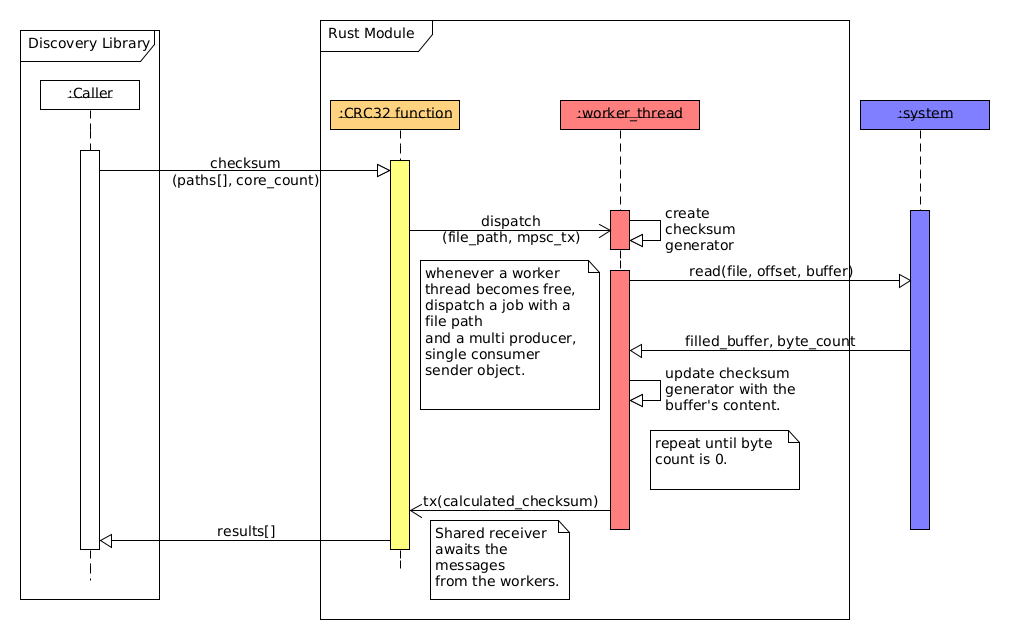
\includegraphics[width=12cm]{figures/checksum/simple_multi_crc}
    \caption{Sequence diagram for a parallelized checksum function.}
    \label{fig:checksum_fig_4}
\end{figure}

The second opportunity for race conditions is when the results are collected.

Figure ~\ref{fig:checksum_fig_4} shows the general flow of the parallelized CRC32 function.
The communication
between the main thread and the worker threads was implemented by using an MPSC FIFO queue (Multi-producer, single-consumer)
each thread receives a sender object, which is used to push their results into the queue.
Finally, after each job finished, the main thread, using the receiver object collects and returns the results to the caller.

The order, in which the results are collected is irrelevant, as it is easy to extend the above flow to include
the file path alongside the calculated checksum (it was omitted, as these tests are purely for benchmarking purposes).
Therefore, the potential for a race condition when collecting the results is also resolved.

\begin{figure}[h]
    \centering
    \begin{bchart}[step=50,max=400, unit=s]
        \bcbar [label=Original, no paralellization]{307}
        \medskip
        \bcbar[label=2 threads]{210}
        \medskip
        \bcbar[label=4 threads]{201}
        \medskip
        \bcbar[label=8 threads]{203}
        \medskip
        \bcbar[label=16 threads]{209}
        \medskip
    \end{bchart}
    \caption{Performance comparison for various thread counts when running the parallelized CRC32 function.}
    \label{fig:checksum_fig_5}
\end{figure}


The introduction of parallelism, did result in significant performance gains ~\ref{fig:checksum_fig_5}.
It is interesting to note, that when the thread count was above four, the performance started to decrease again.
A possible explanation for this is that the test computer has a four core processor, so it is possible that number of context
switching significantly increases after the thread count exceeds the core count (although this explanation
ignores hyper-threading).

\subsection{The IO Problem}
Calculating checksums is a relatively efficient process, to the point that
some processor instruction sets even include CRC32
as a built-in instruction. ~\cite{CRC32Instruction}.

The main bottlenecks therefore, are the IO operations.
This bottleneck becomes apparent when multiple checksums are calculated in parallel.
This is especially true when the files are stored on a hard-drive ~\cite{PiotrParallelDiskAccess}.

Essentially, the threads are competing for the same resource (disk access), slowing each other down.

\begin{figure}[h]
    \centering
    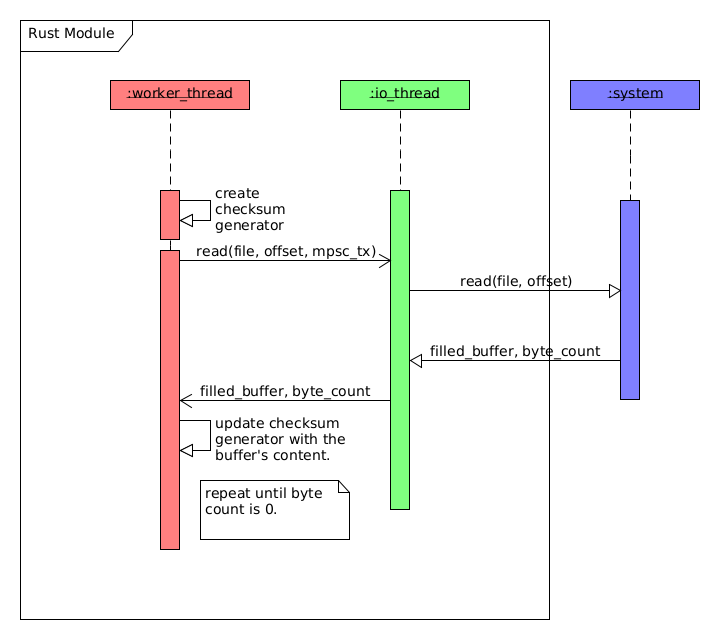
\includegraphics[width=12cm]{figures/checksum/io_multi_crc}
    \caption{Multithreaded CRC32 function, with dedicated IO thread.}
    \label{fig:checksum_fig_6}
\end{figure}

A common solution is to introduce a dedicated IO thread (shown on ~\ref{fig:checksum_fig_6}), from which, each worker thread could
receive the next piece of data to process.

\begin{figure}[h]
    \centering
    \begin{bchart}[step=50,max=400, unit=s]
        \bcbar[label=2 threads]{375}
        \medskip
        \bcbar[label=4 threads]{352}
        \medskip
        \bcbar[label=8 threads]{351}
        \medskip
        \bcbar[label=16 threads]{348}
        \medskip
    \end{bchart}
    \caption{Parallelized CRC32 calculations with dedicated IO thread}
    \label{fig:checksum_fig_7}
\end{figure}


This approach, as it is apparent from the results on ~\ref{fig:checksum_fig_7} caused considerable slow downs,
even compared to single threaded performance.

This slow down, first, can be attributed to increased context switching.
Second, it was also implemented using MPSC queues.
While these queues are great to send simple values back and forth, they were inefficient
when they were used to pass along large buffers, as each time the buffer was sent to the queue,
it had to be copied from the original memory location.

A solution to the latter would be to reimplement the inter-thread communication with shared memory buffers.


\subsection{Solving the IO problem with io\_uring}
Instead of reimplementing ~\ref{fig:checksum_fig_6} with shared memory buffers, an alternative
solution was implemented.

Io\_uring ~\cite{IO_uring} is a novel way of performing asynchronous IO on Linux.
It also claims to increase the performance of multithreaded IO processes.

It relies on two queues, a submission queue (SQ) and a completion queue.
The client simply passes a submission queue entry (SQE), containing the buffer to be filled,
the target file and the offset.

This submission system call is non-blocking, therefore the client may perform other operations
while the system completes the request.
When the client is ready to consume the results,
it can access them from the CQ\@.

\begin{figure}[!htb]
    \centering
    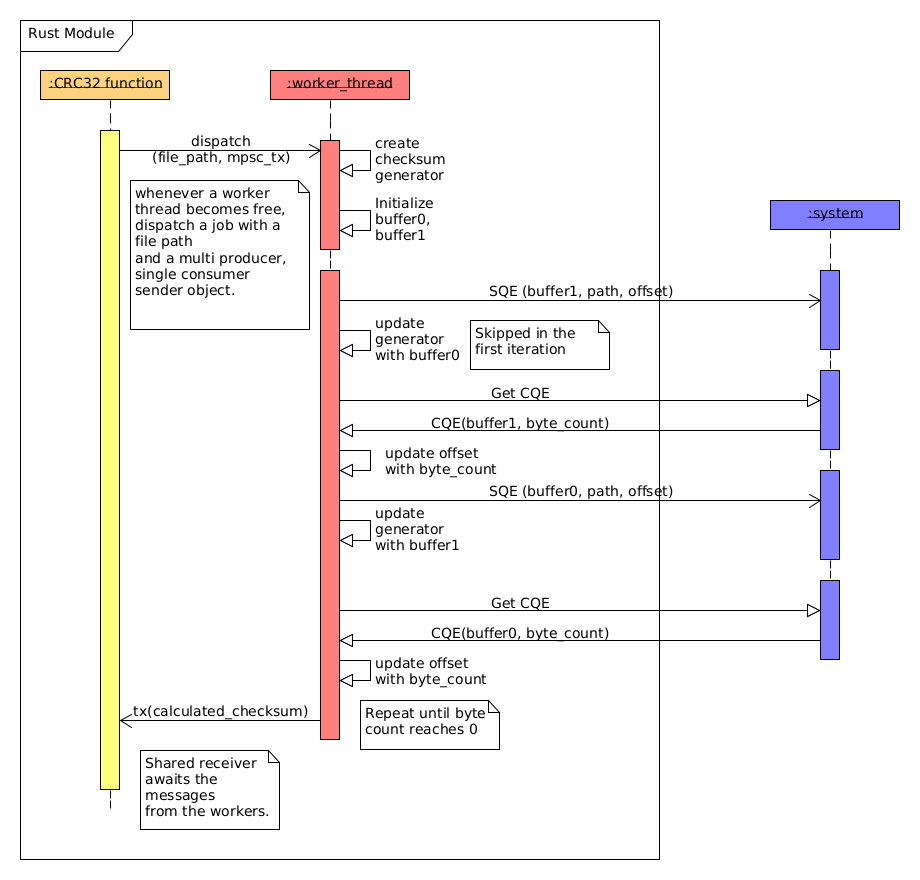
\includegraphics[width=12cm]{figures/checksum/uring_multi_crc}
    \caption{Implementation of the CRC32 function using io\_uring.}
    \label{fig:checksum_fig_8}
\end{figure}

The great benefit of async IO is (as shown on ~\ref{fig:checksum_fig_8}) is that worker threads
don't have to stay idle until the read operation completes.

This behaviour was achieved using a pair of buffers, where one buffer gets processed, while
the other gets refilled.

\begin{figure}[!htb]
    \centering
    \begin{bchart}[step=50,max=400, unit=s]
        \bcbar[label=2 threads]{213}
        \medskip
        \bcbar[label=4 threads]{197}
        \medskip
        \bcbar[label=8 threads]{202}
        \medskip
        \bcbar[label=16 threads]{206}
        \medskip
    \end{bchart}
    \caption{Parallelized CRC32 calculations using io\_uring.}
    \label{fig:checksum_fig_9}
\end{figure}

Some, minor improvements were achieved (~\ref{fig:checksum_fig_9}), but its results were comparable
to the simple, parallelized approach.
This may be attributed to the implementational overhead of using io\_uring.
Alternatively, it is possible that it wasn't designed to be used in such a way, and with
a different approach it could provide greater improvements.

Finally, these benchmarks were executed on an SSD, which perform better when accessed in parallel.
It is probable that, when ran on mechanical hard disk, the usage of io\_uring would achieve
greater differences compared to the original parallel approach.
\clearpage
\subsection{Conclusion}
First, these solutions are not fully optimized.
There are countless ways to shave off a few seconds from each implementation.
They do, however show the general benefits of various approaches.

Second, it is apparent that in the long term, checksums alone won't be sufficient to identify files.
First, the birthday problem virtually guarantees that eventually a collision will happen,
especially when larger filesets are to be considered.

From this issue, even hash functions are not exempt,
since, for example the digest of two empty files will be the same.
The checksum approach however, is still more than sufficient to identify changes across runs,
in the context of individual files.

In the future it would be desirable to attempt using the io\_uring feature again
(especially when there is wider support available), and to include hashing functions
in the benchmarks, as it is possible that their decrease in calculation speeds are
a non-factor when the slow IO performance is considered.

